% Semantic ORDER BY framework figure (Algo1).
% Native width is acmart sigconf textwidth (506.295pt = 177.94mm), probed
% after \maketitle with viz/tex/vendor/acmart.cls + pvldb.sty. Not a new template.
%
% Edge contract. Every edge starts and ends on a border. Solid ink = data.
% Teal dash = control. Red dash is a call-scope box, not an arrow.
%
% D1  c1.south -> call1.north     data   unsorted C1
% D2  c2.south -> call2.north     data   unsorted C2
% D3  c3.south -> call3.north     data   unsorted C3
% D4  c4.south -> call4.north     data   unsorted C4
% D5  call1.south -> g1 north     data   sorted run R1
% D6  call2.south -> g1 north     data   sorted run R2
% D7  call3.south -> g2 north     data   sorted run R3
% D8  call4.south -> g2 north     data   sorted run R4
% D9  g1.south east -> len.north   data   lengths of the left pair
% D10 g2.south west -> len.north   data   lengths of the right pair
% D11 len.south -> est.north      data   |R_i|
% D12 prof.south -> est.north     data   measured profile (H, L)
% C1  mpin.south -> est.north     control  capacity m
% C2  dem.south -> est.north      control  demand mode
% C3  est south-west -> mgL.east  control  (k, h) into left MergeGroup
% C4  est south-east -> mgR.west  control  (k, h) into right MergeGroup
% C5  est south -> mg2.north      control  same (k, h) into pass 2
% C6  C5 branch -> note.north     control  same demand mode, at the output
% D13 mgL.south -> q1.north       data   merged Q1
% D14 mgR.south -> q2.north       data   merged Q2
% D15 q1.south east -> mg2.north   data   Q1 into pass 2
% D16 q2.south west -> mg2.north   data   Q2 into pass 2
% D17 mg2.south -> above Pi        data   element sequence into Pi
%
% finite.py is not drawn. h is not given a fabricated number.
% The drawn pairing is this example's k=2, carried on the control edges.
\documentclass[tikz,border=0pt]{standalone}
\usetikzlibrary{arrows.meta,calc}
\usepackage{amsmath}

\definecolor{ink}{HTML}{1A1A1A}
\definecolor{callfill}{HTML}{F6D7A4}
\definecolor{calledge}{HTML}{D06A12}
\definecolor{callred}{HTML}{C23B2E}
\definecolor{emitblue}{HTML}{1A4E86}
\definecolor{ctrl}{HTML}{0C5C62}
\definecolor{estfill}{HTML}{E5F1F1}
\definecolor{estedge}{HTML}{0C5C62}

\begin{document}
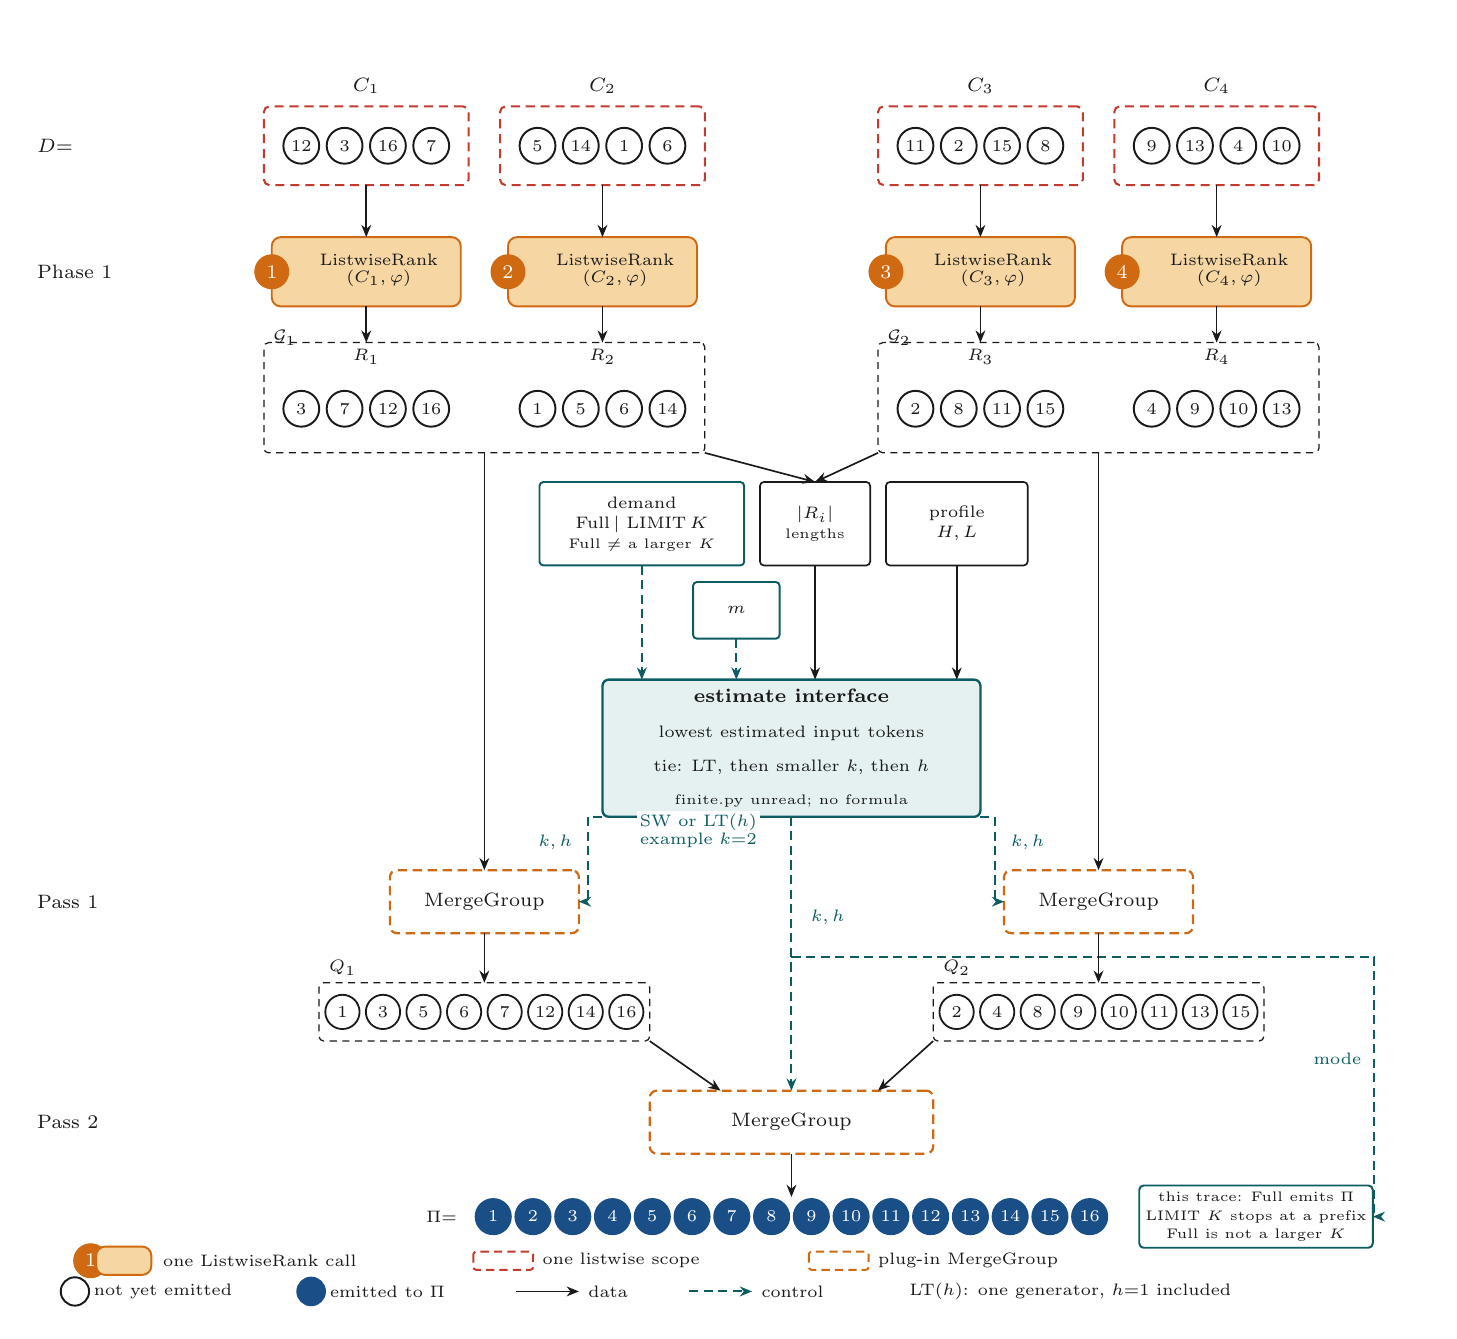
\begin{tikzpicture}[
  x=1mm,y=1mm,
  every node/.style={inner sep=0pt,outer sep=0pt},
  pending/.style={circle,minimum size=4.55mm,inner sep=0pt,fill=white,draw=ink,line width=0.7pt,font=\fontsize{6.4}{7.2}\selectfont,text=ink},
  emitted/.style={circle,minimum size=4.55mm,inner sep=0pt,fill=emitblue,draw=emitblue,line width=0.45pt,font=\fontsize{6.4}{7.2}\selectfont,text=white},
  qchip/.style={circle,minimum size=4.35mm,inner sep=0pt,fill=white,draw=ink,line width=0.65pt,font=\fontsize{6.1}{6.8}\selectfont,text=ink},
  cscope/.style={draw=callred,line width=0.75pt,dash pattern=on 1.15mm off 0.75mm,rounded corners=0.7mm,inner sep=0pt},
  callbox/.style={draw=calledge,fill=callfill,line width=0.7pt,rounded corners=1.15mm,inner sep=0pt},
  badge/.style={circle,minimum size=4.3mm,inner sep=0pt,fill=calledge,draw=calledge,font=\fontsize{6.6}{7}\selectfont\bfseries,text=white},
  groupbox/.style={draw=ink,line width=0.45pt,dash pattern=on 0.9mm off 0.7mm,rounded corners=0.6mm,inner sep=0pt},
  plugin/.style={draw=calledge,line width=0.8pt,dash pattern=on 1.2mm off 0.7mm,rounded corners=0.9mm,fill=white,inner sep=0pt,font=\fontsize{6.6}{7.4}\selectfont,text=ink},
  estbox/.style={draw=estedge,line width=0.85pt,fill=estfill,rounded corners=0.8mm,inner sep=1.2mm,align=center,text=ink},
  pin/.style={draw=ink,line width=0.6pt,fill=white,rounded corners=0.5mm,inner sep=0.7mm,align=center,font=\fontsize{6}{7}\selectfont,text=ink},
  pinctrl/.style={pin,draw=ctrl,line width=0.7pt},
  dat/.style={-{Stealth[length=1.55mm,width=1.25mm]},draw=ink,line width=0.6pt},
  ctl/.style={-{Stealth[length=1.55mm,width=1.25mm]},draw=ctrl,line width=0.75pt,dash pattern=on 1.15mm off 0.7mm},
  lab/.style={font=\fontsize{7.2}{8}\selectfont,text=ink,inner sep=0pt},
  slab/.style={font=\fontsize{6}{7}\selectfont,text=ink,inner sep=0pt}
]
\useasboundingbox (0,0) rectangle (177.94,163);

% ---------- Phase 1 chunks. Red dash = one listwise call's scope. ----------
\node[cscope,minimum width=26mm,minimum height=10mm] (c1) at (43,148) {};
\node[cscope,minimum width=26mm,minimum height=10mm] (c2) at (73,148) {};
\node[cscope,minimum width=26mm,minimum height=10mm] (c3) at (121,148) {};
\node[cscope,minimum width=26mm,minimum height=10mm] (c4) at (151,148) {};
\node[lab] at (43,155.6) {$C_1$};
\node[lab] at (73,155.6) {$C_2$};
\node[lab] at (121,155.6) {$C_3$};
\node[lab] at (151,155.6) {$C_4$};
\node[lab,anchor=west] at (1.2,148) {$D{=}$};

\foreach \x/\n in {34.75/12,40.25/3,45.75/16,51.25/7}
  \node[pending] at (\x,148) {\n};
\foreach \x/\n in {64.75/5,70.25/14,75.75/1,81.25/6}
  \node[pending] at (\x,148) {\n};
\foreach \x/\n in {112.75/11,118.25/2,123.75/15,129.25/8}
  \node[pending] at (\x,148) {\n};
\foreach \x/\n in {142.75/9,148.25/13,153.75/4,159.25/10}
  \node[pending] at (\x,148) {\n};

% ---------- Numbered ListwiseRank calls. Not used on MergeGroup. ----------
\node[callbox,minimum width=24mm,minimum height=8.8mm] (call1) at (43,132) {};
\node[callbox,minimum width=24mm,minimum height=8.8mm] (call2) at (73,132) {};
\node[callbox,minimum width=24mm,minimum height=8.8mm] (call3) at (121,132) {};
\node[callbox,minimum width=24mm,minimum height=8.8mm] (call4) at (151,132) {};
\node[badge] at (call1.west) {$1$};
\node[badge] at (call2.west) {$2$};
\node[badge] at (call3.west) {$3$};
\node[badge] at (call4.west) {$4$};
\node[font=\fontsize{5.7}{6.5}\selectfont,align=center,text=ink] at (44.6,132.15) {ListwiseRank\\[-0.4pt]$(C_1,\varphi)$};
\node[font=\fontsize{5.7}{6.5}\selectfont,align=center,text=ink] at (74.6,132.15) {ListwiseRank\\[-0.4pt]$(C_2,\varphi)$};
\node[font=\fontsize{5.7}{6.5}\selectfont,align=center,text=ink] at (122.6,132.15) {ListwiseRank\\[-0.4pt]$(C_3,\varphi)$};
\node[font=\fontsize{5.7}{6.5}\selectfont,align=center,text=ink] at (152.6,132.15) {ListwiseRank\\[-0.4pt]$(C_4,\varphi)$};
\node[lab,anchor=west] at (1.2,132) {Phase 1};

% ---------- Runs. Hollow = not yet emitted. ----------
\node[groupbox,minimum width=56mm,minimum height=14mm] (g1) at (58,116) {};
\node[groupbox,minimum width=56mm,minimum height=14mm] (g2) at (136,116) {};
\node[slab] at (43,121.2) {$R_1$};
\node[slab] at (73,121.2) {$R_2$};
\node[slab] at (121,121.2) {$R_3$};
\node[slab] at (151,121.2) {$R_4$};
\node[slab,anchor=west] at (31.2,123.6) {$\mathcal{G}_1$};
\node[slab,anchor=west] at (109.2,123.6) {$\mathcal{G}_2$};
\foreach \x/\n in {34.75/3,40.25/7,45.75/12,51.25/16}
  \node[pending] at (\x,114.6) {\n};
\foreach \x/\n in {64.75/1,70.25/5,75.75/6,81.25/14}
  \node[pending] at (\x,114.6) {\n};
\foreach \x/\n in {112.75/2,118.25/8,123.75/11,129.25/15}
  \node[pending] at (\x,114.6) {\n};
\foreach \x/\n in {142.75/4,148.25/9,153.75/10,159.25/13}
  \node[pending] at (\x,114.6) {\n};

% ---------- Inputs of the estimate interface. Above the box, between the data corridors x=58 and x=136. ----------
\node[pinctrl,minimum width=26mm,minimum height=10.6mm] (dem) at (78,100) {demand\\[0.3pt]Full\,$|$\ LIMIT\,$K$\\[0.2pt]{\fontsize{5.5}{6.2}\selectfont Full $\neq$ a larger $K$}};
\node[pin,minimum width=14mm,minimum height=10.6mm] (len) at (100,100) {$|R_i|$\\[0.2pt]{\fontsize{5.5}{6.2}\selectfont lengths}};
\node[pin,minimum width=18mm,minimum height=10.6mm] (prof) at (118,100) {profile\\[0.2pt]$H,L$};
\node[pinctrl,minimum width=11mm,minimum height=7.2mm] (mpin) at (90,89) {$m$};

% ---------- Estimate interface. Policy text is from select_parameters. No finite.py formula. ----------
\node[estbox,minimum width=48mm,minimum height=16.5mm,anchor=north] (est) at (97,80.2) {%
  {\fontsize{7}{8}\selectfont\bfseries estimate interface}\\[0.6pt]
  {\fontsize{5.8}{6.8}\selectfont lowest estimated input tokens}\\[0.15pt]
  {\fontsize{5.8}{6.8}\selectfont tie: LT, then smaller $k$, then $h$}\\[0.15pt]
  {\fontsize{5.5}{6.4}\selectfont finite.py unread; no formula}};

% ---------- Pass 1 plugins. ----------
\node[plugin,minimum width=24mm,minimum height=8mm] (mgL) at (58,52) {MergeGroup};
\node[plugin,minimum width=24mm,minimum height=8mm] (mgR) at (136,52) {MergeGroup};
\node[lab,anchor=west] at (1.2,52) {Pass 1};

% ---------- Q rows. ----------
\node[groupbox,minimum width=42mm,minimum height=7.4mm] (q1) at (58,38) {};
\node[groupbox,minimum width=42mm,minimum height=7.4mm] (q2) at (136,38) {};
\node[slab] at (40,43.6) {$Q_1$};
\node[slab] at (118,43.6) {$Q_2$};
\foreach \i/\n in {0/1,1/3,2/5,3/6,4/7,5/12,6/14,7/16}
  \node[qchip] at ({58-18.025+5.15*\i},38) {\n};
\foreach \i/\n in {0/2,1/4,2/8,3/9,4/10,5/11,6/13,7/15}
  \node[qchip] at ({136-18.025+5.15*\i},38) {\n};

% ---------- Pass 2 plugin and Pi. ----------
\node[plugin,minimum width=36mm,minimum height=8mm] (mg2) at (97,24) {MergeGroup};
\node[lab,anchor=west] at (1.2,24) {Pass 2};
\node[slab,anchor=east] at (54.5,12) {$\Pi{=}$};
\foreach \i in {1,...,16}
  \node[emitted] at ({59.125+5.05*(\i-1)},12) {\i};

\node[draw=ctrl,line width=0.7pt,rounded corners=0.55mm,fill=white,align=center,inner sep=0.8mm,font=\fontsize{5.5}{6.5}\selectfont,text=ink] (note) at (156,12) {this trace: Full emits $\Pi$\\[0.3pt]LIMIT $K$ stops at a prefix\\[0.2pt]{\fontsize{5.5}{6.2}\selectfont Full is not a larger $K$}};

% Selector output sits in the gap under the interface, off the control spine.
\node[align=center,font=\fontsize{5.6}{6.5}\selectfont,text=ctrl,fill=white,inner sep=0.4mm,anchor=east] (fam) at (93,61) {SW or LT($h$)\\[-0.2pt]example $k{=}2$};

% ===================== edges =====================
% Data: elements through Phase 1.
\draw[dat] (c1.south) -- (call1.north);
\draw[dat] (c2.south) -- (call2.north);
\draw[dat] (c3.south) -- (call3.north);
\draw[dat] (c4.south) -- (call4.north);
\draw[dat] (call1.south) -- (43,123);
\draw[dat] (call2.south) -- (73,123);
\draw[dat] (call3.south) -- (121,123);
\draw[dat] (call4.south) -- (151,123);

% Data: run lengths into the interface. Start on the group-box corners.
\draw[dat] (g1.south east) -- (len.north);
\draw[dat] (g2.south west) -- (len.north);
\draw[dat] (len.south) -- (100,80.2);
\draw[dat] (prof.south) -- (118,80.2);

% Control inputs. m is left of the length arrow; demand is left of m.
\draw[ctl] (mpin.south) -- (90,80.2);
\draw[ctl] (dem.south) -- (78,80.2);

% Control outputs leave the south border and stay off the data spines (x=58, x=136).
\draw[ctl] (est.south west) -- ++(-1.8,0) |- (mgL.east);
\draw[ctl] (est.south east) -- ++(1.8,0) |- (mgR.west);
\draw[ctl] (est.south) -- (mg2.north);
\node[slab,text=ctrl,fill=white,inner sep=0.3mm] at ($(est.south west)+(-6,-3.2)$) {$k,h$};
\node[slab,text=ctrl,fill=white,inner sep=0.3mm] at ($(est.south east)+(6,-3.2)$) {$k,h$};
\node[slab,text=ctrl,fill=white,inner sep=0.3mm,anchor=west] at (99.2,50) {$k,h$};

% Mode leaves the same control spine in the open band between Pass 1 and the Q row,
% then drops in the right gutter so it does not enter a box.
\draw[ctl] (97,45) -- (171,45) |- (note.east);
\node[slab,text=ctrl,fill=white,inner sep=0.25mm,anchor=east] at (169.6,32) {mode};

% Data: merge results. The Q-gap element arrow is x=90, beside control x=106.
\draw[dat] (mgL.south) -- (q1.north);
\draw[dat] (mgR.south) -- (q2.north);
\draw[dat] (q1.south east) -- (88,28);
\draw[dat] (q2.south west) -- (108,28);
\draw[dat] (mg2.south) -- (97,14.5);

% Data spines from the run groups into the plugins. x=58 and x=136 miss the estimator (x=73..121).
\draw[dat] (g1.south) -- (mgL.north);
\draw[dat] (g2.south) -- (mgR.north);

% ---------- Legend ----------
\node[badge] at (8,6.4) {$1$};
\node[callbox,minimum width=7mm,minimum height=3.6mm] at (12.2,6.4) {};
\node[slab,anchor=west] at (17.2,6.4) {one ListwiseRank call};
\draw[callred,line width=0.7pt,dash pattern=on 1.05mm off 0.65mm,rounded corners=0.35mm] (56.6,7.55) rectangle (64.2,5.25);
\node[slab,anchor=west] at (65.4,6.4) {one listwise scope};
\draw[calledge,line width=0.7pt,dash pattern=on 1.05mm off 0.65mm,rounded corners=0.35mm] (99.2,7.55) rectangle (106.8,5.25);
\node[slab,anchor=west] at (108,6.4) {plug-in MergeGroup};
\node[pending,minimum size=3.6mm] at (6,2.5) {};
\node[slab,anchor=west] at (8.4,2.5) {not yet emitted};
\node[emitted,minimum size=3.6mm] at (36,2.5) {};
\node[slab,anchor=west] at (38.4,2.5) {emitted to $\Pi$};
\draw[dat] (62,2.5) -- (70,2.5);
\node[slab,anchor=west] at (71.2,2.5) {data};
\draw[ctl] (84,2.5) -- (92,2.5);
\node[slab,anchor=west] at (93.2,2.5) {control};
\node[slab,anchor=west] at (112,2.5) {LT($h$): one generator, $h{=}1$ included};
\end{tikzpicture}
\end{document}
